\documentclass{book}
\usepackage[a4paper,top=2.5cm,bottom=2.5cm,left=2.5cm,right=2.5cm]{geometry}
\usepackage{makeidx}
\usepackage{natbib}
\usepackage{graphicx}
\usepackage{multicol}
\usepackage{float}
\usepackage{listings}
\usepackage{color}
\usepackage{ifthen}
\usepackage[table]{xcolor}
\usepackage{textcomp}
\usepackage{alltt}
\usepackage{ifpdf}
\ifpdf
\usepackage[pdftex,
            pagebackref=true,
            colorlinks=true,
            linkcolor=blue,
            unicode
           ]{hyperref}
\else
\usepackage[ps2pdf,
            pagebackref=true,
            colorlinks=true,
            linkcolor=blue,
            unicode
           ]{hyperref}
\usepackage{pspicture}
\fi
\usepackage[utf8]{inputenc}
\usepackage{mathptmx}
\usepackage[scaled=.90]{helvet}
\usepackage{courier}
\usepackage{sectsty}
\usepackage{amssymb}
\usepackage[titles]{tocloft}
\usepackage{doxygen}
\lstset{language=C++,inputencoding=utf8,basicstyle=\footnotesize,breaklines=true,breakatwhitespace=true,tabsize=4,numbers=left }
\makeindex
\setcounter{tocdepth}{3}
\renewcommand{\footrulewidth}{0.4pt}
\renewcommand{\familydefault}{\sfdefault}
\hfuzz=15pt
\setlength{\emergencystretch}{15pt}
\hbadness=750
\tolerance=750
\begin{document}
\hypersetup{pageanchor=false,citecolor=blue}
\begin{titlepage}
\vspace*{7cm}
\begin{center}
{\Large H\-O\-S\-T Activity Testing \\[1ex]\large 1 }\\
\vspace*{1cm}
{\large Generated by Doxygen 1.8.3.1}\\
\vspace*{0.5cm}
{\small Wed Apr 24 2013 21:20:29}\\
\end{center}
\end{titlepage}
\clearemptydoublepage
\pagenumbering{roman}
\tableofcontents
\clearemptydoublepage
\pagenumbering{arabic}
\hypersetup{pageanchor=true,citecolor=blue}
\chapter{Hierarchical Index}
\section{Class Hierarchy}
This inheritance list is sorted roughly, but not completely, alphabetically\-:\begin{DoxyCompactList}
\item Activity\-Instrumentation\-Test\-Case2\begin{DoxyCompactList}
\item \contentsline{section}{org.\-habitatomaha.\-H\-O\-S\-T.\-Activity.\-Select\-Form\-Activity\-Test}{\pageref{classorg_1_1habitatomaha_1_1_h_o_s_t_1_1_activity_1_1_select_form_activity_test}}{}
\end{DoxyCompactList}
\item Activity\-Unit\-Test\-Case\begin{DoxyCompactList}
\item \contentsline{section}{org.\-habitatomaha.\-H\-O\-S\-T.\-Activity.\-Edit\-Form\-Activity\-Test}{\pageref{classorg_1_1habitatomaha_1_1_h_o_s_t_1_1_activity_1_1_edit_form_activity_test}}{}
\item \contentsline{section}{org.\-habitatomaha.\-H\-O\-S\-T.\-Activity.\-Submit\-Form\-Activity\-Test}{\pageref{classorg_1_1habitatomaha_1_1_h_o_s_t_1_1_activity_1_1_submit_form_activity_test}}{}
\end{DoxyCompactList}
\end{DoxyCompactList}

\chapter{Class Index}
\section{Class List}
Here are the classes, structs, unions and interfaces with brief descriptions\-:\begin{DoxyCompactList}
\item\contentsline{section}{\hyperlink{classorg_1_1habitatomaha_1_1_h_o_s_t_1_1_activity_1_1_edit_form_activity_test}{org.\-habitatomaha.\-H\-O\-S\-T.\-Activity.\-Edit\-Form\-Activity\-Test} }{\pageref{classorg_1_1habitatomaha_1_1_h_o_s_t_1_1_activity_1_1_edit_form_activity_test}}{}
\item\contentsline{section}{\hyperlink{classorg_1_1habitatomaha_1_1_h_o_s_t_1_1_activity_1_1_select_form_activity_test}{org.\-habitatomaha.\-H\-O\-S\-T.\-Activity.\-Select\-Form\-Activity\-Test} }{\pageref{classorg_1_1habitatomaha_1_1_h_o_s_t_1_1_activity_1_1_select_form_activity_test}}{}
\item\contentsline{section}{\hyperlink{classorg_1_1habitatomaha_1_1_h_o_s_t_1_1_activity_1_1_submit_form_activity_test}{org.\-habitatomaha.\-H\-O\-S\-T.\-Activity.\-Submit\-Form\-Activity\-Test} }{\pageref{classorg_1_1habitatomaha_1_1_h_o_s_t_1_1_activity_1_1_submit_form_activity_test}}{}
\end{DoxyCompactList}

\chapter{Class Documentation}
\hypertarget{classorg_1_1habitatomaha_1_1_h_o_s_t_1_1_activity_1_1_edit_form_activity_test}{\section{org.\-habitatomaha.\-H\-O\-S\-T.\-Activity.\-Edit\-Form\-Activity\-Test Class Reference}
\label{classorg_1_1habitatomaha_1_1_h_o_s_t_1_1_activity_1_1_edit_form_activity_test}\index{org.\-habitatomaha.\-H\-O\-S\-T.\-Activity.\-Edit\-Form\-Activity\-Test@{org.\-habitatomaha.\-H\-O\-S\-T.\-Activity.\-Edit\-Form\-Activity\-Test}}
}
Inheritance diagram for org.\-habitatomaha.\-H\-O\-S\-T.\-Activity.\-Edit\-Form\-Activity\-Test\-:\begin{figure}[H]
\begin{center}
\leavevmode
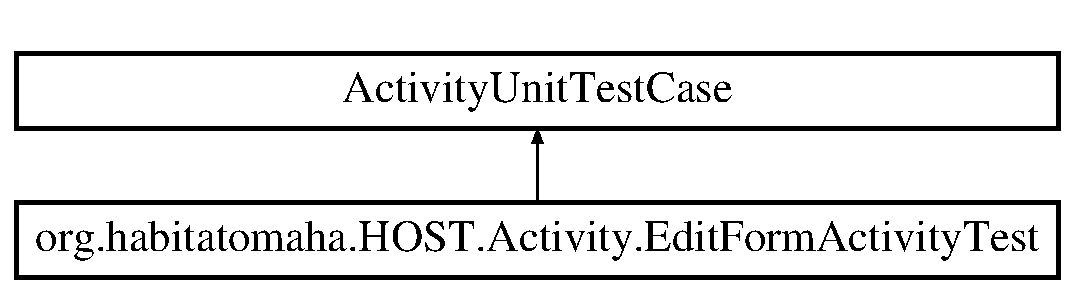
\includegraphics[height=2.000000cm]{classorg_1_1habitatomaha_1_1_h_o_s_t_1_1_activity_1_1_edit_form_activity_test}
\end{center}
\end{figure}
\subsection*{Public Member Functions}
\begin{DoxyCompactItemize}
\item 
\hyperlink{classorg_1_1habitatomaha_1_1_h_o_s_t_1_1_activity_1_1_edit_form_activity_test_a841881fa137d0a3558fa2c92846ba465}{Edit\-Form\-Activity\-Test} ()
\item 
void \hyperlink{classorg_1_1habitatomaha_1_1_h_o_s_t_1_1_activity_1_1_edit_form_activity_test_a05d4058b86b484f9b770b337d8c1e61f}{test\-Life\-Cycle\-Create} ()
\item 
void \hyperlink{classorg_1_1habitatomaha_1_1_h_o_s_t_1_1_activity_1_1_edit_form_activity_test_acda7c44bcd3aeebc79f0ca535d5e9c70}{test\-Pre\-Conditions} ()
\item 
\hypertarget{classorg_1_1habitatomaha_1_1_h_o_s_t_1_1_activity_1_1_edit_form_activity_test_adda5892e7f067d8c775371ad9a58f20d}{void {\bfseries example\-Activity\-Test\-N\-O\-T\-U\-S\-E\-D} ()}\label{classorg_1_1habitatomaha_1_1_h_o_s_t_1_1_activity_1_1_edit_form_activity_test_adda5892e7f067d8c775371ad9a58f20d}

\item 
\hypertarget{classorg_1_1habitatomaha_1_1_h_o_s_t_1_1_activity_1_1_edit_form_activity_test_a2635a802cb9229c01f3e60fd107a8584}{void {\bfseries test\-State\-Destroy} ()}\label{classorg_1_1habitatomaha_1_1_h_o_s_t_1_1_activity_1_1_edit_form_activity_test_a2635a802cb9229c01f3e60fd107a8584}

\item 
\hypertarget{classorg_1_1habitatomaha_1_1_h_o_s_t_1_1_activity_1_1_edit_form_activity_test_a7f5b27ab3928842373c036af132a7c8b}{void {\bfseries test\-State\-Pause} ()}\label{classorg_1_1habitatomaha_1_1_h_o_s_t_1_1_activity_1_1_edit_form_activity_test_a7f5b27ab3928842373c036af132a7c8b}

\end{DoxyCompactItemize}
\subsection*{Protected Member Functions}
\begin{DoxyCompactItemize}
\item 
void \hyperlink{classorg_1_1habitatomaha_1_1_h_o_s_t_1_1_activity_1_1_edit_form_activity_test_acf343fd365da6456c23310bb1d2b3520}{set\-Up} ()  throws Exception 
\item 
void \hyperlink{classorg_1_1habitatomaha_1_1_h_o_s_t_1_1_activity_1_1_edit_form_activity_test_a693e8215981053a50ec0f2ae91995178}{tear\-Down} ()  throws Exception
\end{DoxyCompactItemize}


\subsection{Constructor \& Destructor Documentation}
\hypertarget{classorg_1_1habitatomaha_1_1_h_o_s_t_1_1_activity_1_1_edit_form_activity_test_a841881fa137d0a3558fa2c92846ba465}{\index{org\-::habitatomaha\-::\-H\-O\-S\-T\-::\-Activity\-::\-Edit\-Form\-Activity\-Test@{org\-::habitatomaha\-::\-H\-O\-S\-T\-::\-Activity\-::\-Edit\-Form\-Activity\-Test}!Edit\-Form\-Activity\-Test@{Edit\-Form\-Activity\-Test}}
\index{Edit\-Form\-Activity\-Test@{Edit\-Form\-Activity\-Test}!org::habitatomaha::HOST::Activity::EditFormActivityTest@{org\-::habitatomaha\-::\-H\-O\-S\-T\-::\-Activity\-::\-Edit\-Form\-Activity\-Test}}
\subsubsection[{Edit\-Form\-Activity\-Test}]{\setlength{\rightskip}{0pt plus 5cm}org.\-habitatomaha.\-H\-O\-S\-T.\-Activity.\-Edit\-Form\-Activity\-Test.\-Edit\-Form\-Activity\-Test (
\begin{DoxyParamCaption}
{}
\end{DoxyParamCaption}
)}}\label{classorg_1_1habitatomaha_1_1_h_o_s_t_1_1_activity_1_1_edit_form_activity_test_a841881fa137d0a3558fa2c92846ba465}
a Constructor is needed for Android based Unit tests and Activity tests 

\subsection{Member Function Documentation}
\hypertarget{classorg_1_1habitatomaha_1_1_h_o_s_t_1_1_activity_1_1_edit_form_activity_test_acf343fd365da6456c23310bb1d2b3520}{\index{org\-::habitatomaha\-::\-H\-O\-S\-T\-::\-Activity\-::\-Edit\-Form\-Activity\-Test@{org\-::habitatomaha\-::\-H\-O\-S\-T\-::\-Activity\-::\-Edit\-Form\-Activity\-Test}!set\-Up@{set\-Up}}
\index{set\-Up@{set\-Up}!org::habitatomaha::HOST::Activity::EditFormActivityTest@{org\-::habitatomaha\-::\-H\-O\-S\-T\-::\-Activity\-::\-Edit\-Form\-Activity\-Test}}
\subsubsection[{set\-Up}]{\setlength{\rightskip}{0pt plus 5cm}void org.\-habitatomaha.\-H\-O\-S\-T.\-Activity.\-Edit\-Form\-Activity\-Test.\-set\-Up (
\begin{DoxyParamCaption}
{}
\end{DoxyParamCaption}
)  throws Exception \hspace{0.3cm}{\ttfamily [protected]}}}\label{classorg_1_1habitatomaha_1_1_h_o_s_t_1_1_activity_1_1_edit_form_activity_test_acf343fd365da6456c23310bb1d2b3520}
A Setup function is required in order to initialize android components before a test is ran. \hypertarget{classorg_1_1habitatomaha_1_1_h_o_s_t_1_1_activity_1_1_edit_form_activity_test_a693e8215981053a50ec0f2ae91995178}{\index{org\-::habitatomaha\-::\-H\-O\-S\-T\-::\-Activity\-::\-Edit\-Form\-Activity\-Test@{org\-::habitatomaha\-::\-H\-O\-S\-T\-::\-Activity\-::\-Edit\-Form\-Activity\-Test}!tear\-Down@{tear\-Down}}
\index{tear\-Down@{tear\-Down}!org::habitatomaha::HOST::Activity::EditFormActivityTest@{org\-::habitatomaha\-::\-H\-O\-S\-T\-::\-Activity\-::\-Edit\-Form\-Activity\-Test}}
\subsubsection[{tear\-Down}]{\setlength{\rightskip}{0pt plus 5cm}void org.\-habitatomaha.\-H\-O\-S\-T.\-Activity.\-Edit\-Form\-Activity\-Test.\-tear\-Down (
\begin{DoxyParamCaption}
{}
\end{DoxyParamCaption}
)  throws Exception\hspace{0.3cm}{\ttfamily [protected]}}}\label{classorg_1_1habitatomaha_1_1_h_o_s_t_1_1_activity_1_1_edit_form_activity_test_a693e8215981053a50ec0f2ae91995178}
A Tear Down method is necessary to end the test and reset android components \hypertarget{classorg_1_1habitatomaha_1_1_h_o_s_t_1_1_activity_1_1_edit_form_activity_test_a05d4058b86b484f9b770b337d8c1e61f}{\index{org\-::habitatomaha\-::\-H\-O\-S\-T\-::\-Activity\-::\-Edit\-Form\-Activity\-Test@{org\-::habitatomaha\-::\-H\-O\-S\-T\-::\-Activity\-::\-Edit\-Form\-Activity\-Test}!test\-Life\-Cycle\-Create@{test\-Life\-Cycle\-Create}}
\index{test\-Life\-Cycle\-Create@{test\-Life\-Cycle\-Create}!org::habitatomaha::HOST::Activity::EditFormActivityTest@{org\-::habitatomaha\-::\-H\-O\-S\-T\-::\-Activity\-::\-Edit\-Form\-Activity\-Test}}
\subsubsection[{test\-Life\-Cycle\-Create}]{\setlength{\rightskip}{0pt plus 5cm}void org.\-habitatomaha.\-H\-O\-S\-T.\-Activity.\-Edit\-Form\-Activity\-Test.\-test\-Life\-Cycle\-Create (
\begin{DoxyParamCaption}
{}
\end{DoxyParamCaption}
)}}\label{classorg_1_1habitatomaha_1_1_h_o_s_t_1_1_activity_1_1_edit_form_activity_test_a05d4058b86b484f9b770b337d8c1e61f}
Test the lifecycle of the activity to ensure that the activity can be Stopped/\-Started/\-Restarted/\-Paused/closed without an error. \hypertarget{classorg_1_1habitatomaha_1_1_h_o_s_t_1_1_activity_1_1_edit_form_activity_test_acda7c44bcd3aeebc79f0ca535d5e9c70}{\index{org\-::habitatomaha\-::\-H\-O\-S\-T\-::\-Activity\-::\-Edit\-Form\-Activity\-Test@{org\-::habitatomaha\-::\-H\-O\-S\-T\-::\-Activity\-::\-Edit\-Form\-Activity\-Test}!test\-Pre\-Conditions@{test\-Pre\-Conditions}}
\index{test\-Pre\-Conditions@{test\-Pre\-Conditions}!org::habitatomaha::HOST::Activity::EditFormActivityTest@{org\-::habitatomaha\-::\-H\-O\-S\-T\-::\-Activity\-::\-Edit\-Form\-Activity\-Test}}
\subsubsection[{test\-Pre\-Conditions}]{\setlength{\rightskip}{0pt plus 5cm}void org.\-habitatomaha.\-H\-O\-S\-T.\-Activity.\-Edit\-Form\-Activity\-Test.\-test\-Pre\-Conditions (
\begin{DoxyParamCaption}
{}
\end{DoxyParamCaption}
)}}\label{classorg_1_1habitatomaha_1_1_h_o_s_t_1_1_activity_1_1_edit_form_activity_test_acda7c44bcd3aeebc79f0ca535d5e9c70}
Initial state test for the Answer text field.

It cannot be null (properly initialized), it's text value cannot be null (proper answer) and should have the focus on the screen. 

The documentation for this class was generated from the following file\-:\begin{DoxyCompactItemize}
\item 
src/org/habitatomaha/\-H\-O\-S\-T/\-Activity/Edit\-Form\-Activity\-Test.\-java\end{DoxyCompactItemize}

\hypertarget{classorg_1_1habitatomaha_1_1_h_o_s_t_1_1_activity_1_1_select_form_activity_test}{\section{org.\-habitatomaha.\-H\-O\-S\-T.\-Activity.\-Select\-Form\-Activity\-Test Class Reference}
\label{classorg_1_1habitatomaha_1_1_h_o_s_t_1_1_activity_1_1_select_form_activity_test}\index{org.\-habitatomaha.\-H\-O\-S\-T.\-Activity.\-Select\-Form\-Activity\-Test@{org.\-habitatomaha.\-H\-O\-S\-T.\-Activity.\-Select\-Form\-Activity\-Test}}
}
Inheritance diagram for org.\-habitatomaha.\-H\-O\-S\-T.\-Activity.\-Select\-Form\-Activity\-Test\-:\begin{figure}[H]
\begin{center}
\leavevmode
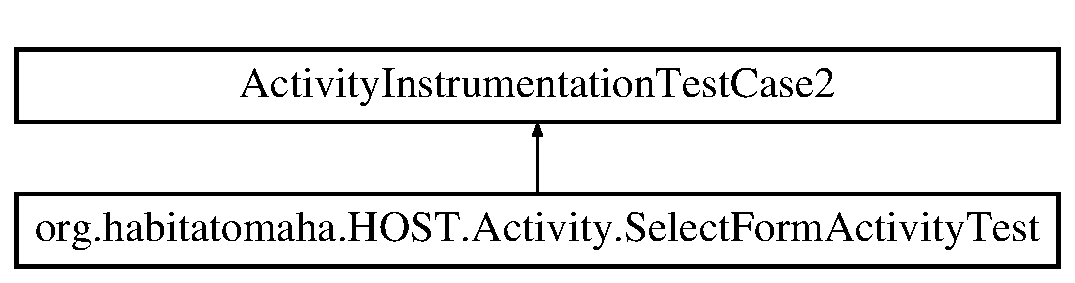
\includegraphics[height=2.000000cm]{classorg_1_1habitatomaha_1_1_h_o_s_t_1_1_activity_1_1_select_form_activity_test}
\end{center}
\end{figure}
\subsection*{Public Member Functions}
\begin{DoxyCompactItemize}
\item 
\hyperlink{classorg_1_1habitatomaha_1_1_h_o_s_t_1_1_activity_1_1_select_form_activity_test_a1c36d3926858cc7a01904e42834637f7}{Select\-Form\-Activity\-Test} ()
\item 
void \hyperlink{classorg_1_1habitatomaha_1_1_h_o_s_t_1_1_activity_1_1_select_form_activity_test_a754c487f825ff9eac17490d90c09cea4}{test\-Pre\-Conditions} ()
\item 
void \hyperlink{classorg_1_1habitatomaha_1_1_h_o_s_t_1_1_activity_1_1_select_form_activity_test_a7918c78326b5258573ebed55d110b2fb}{test\-Life\-Cycle\-Create} ()
\item 
\hypertarget{classorg_1_1habitatomaha_1_1_h_o_s_t_1_1_activity_1_1_select_form_activity_test_a513d12171fd97ac76bc5b6fdd797fb94}{void {\bfseries example\-Activity\-Test\-N\-O\-T\-U\-S\-E\-D} ()}\label{classorg_1_1habitatomaha_1_1_h_o_s_t_1_1_activity_1_1_select_form_activity_test_a513d12171fd97ac76bc5b6fdd797fb94}

\item 
void \hyperlink{classorg_1_1habitatomaha_1_1_h_o_s_t_1_1_activity_1_1_select_form_activity_test_ada1b61c2f7178c212f253d25f9d9abbf}{test\-State\-Destroy} ()
\item 
void \hyperlink{classorg_1_1habitatomaha_1_1_h_o_s_t_1_1_activity_1_1_select_form_activity_test_adcbd145f225f0ab38ea17bf4ae208349}{test\-State\-Pause} ()
\end{DoxyCompactItemize}
\subsection*{Protected Member Functions}
\begin{DoxyCompactItemize}
\item 
void \hyperlink{classorg_1_1habitatomaha_1_1_h_o_s_t_1_1_activity_1_1_select_form_activity_test_a83ee5b9f80bae51a1dbe59b9ee3f3c69}{set\-Up} ()  throws Exception 
\end{DoxyCompactItemize}


\subsection{Constructor \& Destructor Documentation}
\hypertarget{classorg_1_1habitatomaha_1_1_h_o_s_t_1_1_activity_1_1_select_form_activity_test_a1c36d3926858cc7a01904e42834637f7}{\index{org\-::habitatomaha\-::\-H\-O\-S\-T\-::\-Activity\-::\-Select\-Form\-Activity\-Test@{org\-::habitatomaha\-::\-H\-O\-S\-T\-::\-Activity\-::\-Select\-Form\-Activity\-Test}!Select\-Form\-Activity\-Test@{Select\-Form\-Activity\-Test}}
\index{Select\-Form\-Activity\-Test@{Select\-Form\-Activity\-Test}!org::habitatomaha::HOST::Activity::SelectFormActivityTest@{org\-::habitatomaha\-::\-H\-O\-S\-T\-::\-Activity\-::\-Select\-Form\-Activity\-Test}}
\subsubsection[{Select\-Form\-Activity\-Test}]{\setlength{\rightskip}{0pt plus 5cm}org.\-habitatomaha.\-H\-O\-S\-T.\-Activity.\-Select\-Form\-Activity\-Test.\-Select\-Form\-Activity\-Test (
\begin{DoxyParamCaption}
{}
\end{DoxyParamCaption}
)}}\label{classorg_1_1habitatomaha_1_1_h_o_s_t_1_1_activity_1_1_select_form_activity_test_a1c36d3926858cc7a01904e42834637f7}
a Constructor is needed for Android based Unit tests and Activity tests 

\subsection{Member Function Documentation}
\hypertarget{classorg_1_1habitatomaha_1_1_h_o_s_t_1_1_activity_1_1_select_form_activity_test_a83ee5b9f80bae51a1dbe59b9ee3f3c69}{\index{org\-::habitatomaha\-::\-H\-O\-S\-T\-::\-Activity\-::\-Select\-Form\-Activity\-Test@{org\-::habitatomaha\-::\-H\-O\-S\-T\-::\-Activity\-::\-Select\-Form\-Activity\-Test}!set\-Up@{set\-Up}}
\index{set\-Up@{set\-Up}!org::habitatomaha::HOST::Activity::SelectFormActivityTest@{org\-::habitatomaha\-::\-H\-O\-S\-T\-::\-Activity\-::\-Select\-Form\-Activity\-Test}}
\subsubsection[{set\-Up}]{\setlength{\rightskip}{0pt plus 5cm}void org.\-habitatomaha.\-H\-O\-S\-T.\-Activity.\-Select\-Form\-Activity\-Test.\-set\-Up (
\begin{DoxyParamCaption}
{}
\end{DoxyParamCaption}
)  throws Exception \hspace{0.3cm}{\ttfamily [protected]}}}\label{classorg_1_1habitatomaha_1_1_h_o_s_t_1_1_activity_1_1_select_form_activity_test_a83ee5b9f80bae51a1dbe59b9ee3f3c69}
A Setup function is required in order to initialize android components before a test is ran. \hypertarget{classorg_1_1habitatomaha_1_1_h_o_s_t_1_1_activity_1_1_select_form_activity_test_a7918c78326b5258573ebed55d110b2fb}{\index{org\-::habitatomaha\-::\-H\-O\-S\-T\-::\-Activity\-::\-Select\-Form\-Activity\-Test@{org\-::habitatomaha\-::\-H\-O\-S\-T\-::\-Activity\-::\-Select\-Form\-Activity\-Test}!test\-Life\-Cycle\-Create@{test\-Life\-Cycle\-Create}}
\index{test\-Life\-Cycle\-Create@{test\-Life\-Cycle\-Create}!org::habitatomaha::HOST::Activity::SelectFormActivityTest@{org\-::habitatomaha\-::\-H\-O\-S\-T\-::\-Activity\-::\-Select\-Form\-Activity\-Test}}
\subsubsection[{test\-Life\-Cycle\-Create}]{\setlength{\rightskip}{0pt plus 5cm}void org.\-habitatomaha.\-H\-O\-S\-T.\-Activity.\-Select\-Form\-Activity\-Test.\-test\-Life\-Cycle\-Create (
\begin{DoxyParamCaption}
{}
\end{DoxyParamCaption}
)}}\label{classorg_1_1habitatomaha_1_1_h_o_s_t_1_1_activity_1_1_select_form_activity_test_a7918c78326b5258573ebed55d110b2fb}
Test the lifecycle of the activity to ensure that the activity can be Stopped/\-Started/\-Restarted/\-Paused/closed without an error. \hypertarget{classorg_1_1habitatomaha_1_1_h_o_s_t_1_1_activity_1_1_select_form_activity_test_a754c487f825ff9eac17490d90c09cea4}{\index{org\-::habitatomaha\-::\-H\-O\-S\-T\-::\-Activity\-::\-Select\-Form\-Activity\-Test@{org\-::habitatomaha\-::\-H\-O\-S\-T\-::\-Activity\-::\-Select\-Form\-Activity\-Test}!test\-Pre\-Conditions@{test\-Pre\-Conditions}}
\index{test\-Pre\-Conditions@{test\-Pre\-Conditions}!org::habitatomaha::HOST::Activity::SelectFormActivityTest@{org\-::habitatomaha\-::\-H\-O\-S\-T\-::\-Activity\-::\-Select\-Form\-Activity\-Test}}
\subsubsection[{test\-Pre\-Conditions}]{\setlength{\rightskip}{0pt plus 5cm}void org.\-habitatomaha.\-H\-O\-S\-T.\-Activity.\-Select\-Form\-Activity\-Test.\-test\-Pre\-Conditions (
\begin{DoxyParamCaption}
{}
\end{DoxyParamCaption}
)}}\label{classorg_1_1habitatomaha_1_1_h_o_s_t_1_1_activity_1_1_select_form_activity_test_a754c487f825ff9eac17490d90c09cea4}
Initial State Test -\/ what should be true when the app is ran for the first time \hypertarget{classorg_1_1habitatomaha_1_1_h_o_s_t_1_1_activity_1_1_select_form_activity_test_ada1b61c2f7178c212f253d25f9d9abbf}{\index{org\-::habitatomaha\-::\-H\-O\-S\-T\-::\-Activity\-::\-Select\-Form\-Activity\-Test@{org\-::habitatomaha\-::\-H\-O\-S\-T\-::\-Activity\-::\-Select\-Form\-Activity\-Test}!test\-State\-Destroy@{test\-State\-Destroy}}
\index{test\-State\-Destroy@{test\-State\-Destroy}!org::habitatomaha::HOST::Activity::SelectFormActivityTest@{org\-::habitatomaha\-::\-H\-O\-S\-T\-::\-Activity\-::\-Select\-Form\-Activity\-Test}}
\subsubsection[{test\-State\-Destroy}]{\setlength{\rightskip}{0pt plus 5cm}void org.\-habitatomaha.\-H\-O\-S\-T.\-Activity.\-Select\-Form\-Activity\-Test.\-test\-State\-Destroy (
\begin{DoxyParamCaption}
{}
\end{DoxyParamCaption}
)}}\label{classorg_1_1habitatomaha_1_1_h_o_s_t_1_1_activity_1_1_select_form_activity_test_ada1b61c2f7178c212f253d25f9d9abbf}
State Management Test -\/ test if the activity keeps its values after being closed \hypertarget{classorg_1_1habitatomaha_1_1_h_o_s_t_1_1_activity_1_1_select_form_activity_test_adcbd145f225f0ab38ea17bf4ae208349}{\index{org\-::habitatomaha\-::\-H\-O\-S\-T\-::\-Activity\-::\-Select\-Form\-Activity\-Test@{org\-::habitatomaha\-::\-H\-O\-S\-T\-::\-Activity\-::\-Select\-Form\-Activity\-Test}!test\-State\-Pause@{test\-State\-Pause}}
\index{test\-State\-Pause@{test\-State\-Pause}!org::habitatomaha::HOST::Activity::SelectFormActivityTest@{org\-::habitatomaha\-::\-H\-O\-S\-T\-::\-Activity\-::\-Select\-Form\-Activity\-Test}}
\subsubsection[{test\-State\-Pause}]{\setlength{\rightskip}{0pt plus 5cm}void org.\-habitatomaha.\-H\-O\-S\-T.\-Activity.\-Select\-Form\-Activity\-Test.\-test\-State\-Pause (
\begin{DoxyParamCaption}
{}
\end{DoxyParamCaption}
)}}\label{classorg_1_1habitatomaha_1_1_h_o_s_t_1_1_activity_1_1_select_form_activity_test_adcbd145f225f0ab38ea17bf4ae208349}
State management for Pause and Idle states of the Android O\-S.

These tests are required to run off of a U\-I thread due to interaction with the instrumentation 

The documentation for this class was generated from the following file\-:\begin{DoxyCompactItemize}
\item 
src/org/habitatomaha/\-H\-O\-S\-T/\-Activity/Select\-Form\-Activity\-Test.\-java\end{DoxyCompactItemize}

\hypertarget{classorg_1_1habitatomaha_1_1_h_o_s_t_1_1_activity_1_1_submit_form_activity_test}{\section{org.\-habitatomaha.\-H\-O\-S\-T.\-Activity.\-Submit\-Form\-Activity\-Test Class Reference}
\label{classorg_1_1habitatomaha_1_1_h_o_s_t_1_1_activity_1_1_submit_form_activity_test}\index{org.\-habitatomaha.\-H\-O\-S\-T.\-Activity.\-Submit\-Form\-Activity\-Test@{org.\-habitatomaha.\-H\-O\-S\-T.\-Activity.\-Submit\-Form\-Activity\-Test}}
}
Inheritance diagram for org.\-habitatomaha.\-H\-O\-S\-T.\-Activity.\-Submit\-Form\-Activity\-Test\-:\begin{figure}[H]
\begin{center}
\leavevmode
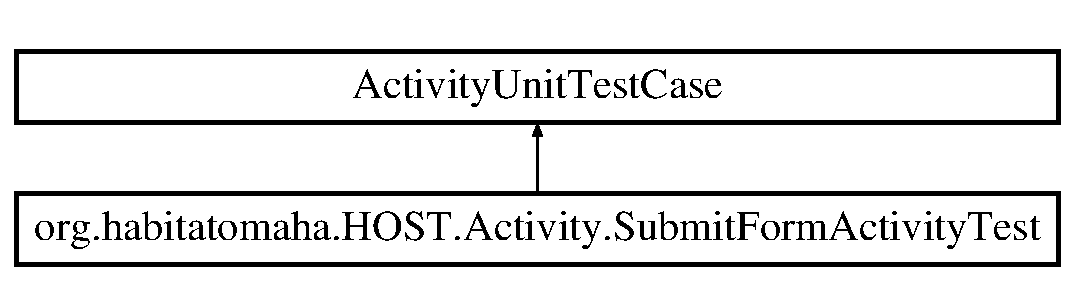
\includegraphics[height=2.000000cm]{classorg_1_1habitatomaha_1_1_h_o_s_t_1_1_activity_1_1_submit_form_activity_test}
\end{center}
\end{figure}
\subsection*{Public Member Functions}
\begin{DoxyCompactItemize}
\item 
\hyperlink{classorg_1_1habitatomaha_1_1_h_o_s_t_1_1_activity_1_1_submit_form_activity_test_acbb130572a8cf5c80a037958e5225a1a}{Submit\-Form\-Activity\-Test} ()
\item 
void \hyperlink{classorg_1_1habitatomaha_1_1_h_o_s_t_1_1_activity_1_1_submit_form_activity_test_ab5d5f6b4c161ad37a4548fc19a82e1b5}{test\-Life\-Cycle\-Create} ()
\end{DoxyCompactItemize}
\subsection*{Protected Member Functions}
\begin{DoxyCompactItemize}
\item 
void \hyperlink{classorg_1_1habitatomaha_1_1_h_o_s_t_1_1_activity_1_1_submit_form_activity_test_a76b52475256cd3465965d9a07d10668d}{set\-Up} ()  throws Exception 
\item 
void \hyperlink{classorg_1_1habitatomaha_1_1_h_o_s_t_1_1_activity_1_1_submit_form_activity_test_a8c5da29be5109dbff7f0ead4eae990dd}{tear\-Down} ()  throws Exception
\end{DoxyCompactItemize}


\subsection{Constructor \& Destructor Documentation}
\hypertarget{classorg_1_1habitatomaha_1_1_h_o_s_t_1_1_activity_1_1_submit_form_activity_test_acbb130572a8cf5c80a037958e5225a1a}{\index{org\-::habitatomaha\-::\-H\-O\-S\-T\-::\-Activity\-::\-Submit\-Form\-Activity\-Test@{org\-::habitatomaha\-::\-H\-O\-S\-T\-::\-Activity\-::\-Submit\-Form\-Activity\-Test}!Submit\-Form\-Activity\-Test@{Submit\-Form\-Activity\-Test}}
\index{Submit\-Form\-Activity\-Test@{Submit\-Form\-Activity\-Test}!org::habitatomaha::HOST::Activity::SubmitFormActivityTest@{org\-::habitatomaha\-::\-H\-O\-S\-T\-::\-Activity\-::\-Submit\-Form\-Activity\-Test}}
\subsubsection[{Submit\-Form\-Activity\-Test}]{\setlength{\rightskip}{0pt plus 5cm}org.\-habitatomaha.\-H\-O\-S\-T.\-Activity.\-Submit\-Form\-Activity\-Test.\-Submit\-Form\-Activity\-Test (
\begin{DoxyParamCaption}
{}
\end{DoxyParamCaption}
)}}\label{classorg_1_1habitatomaha_1_1_h_o_s_t_1_1_activity_1_1_submit_form_activity_test_acbb130572a8cf5c80a037958e5225a1a}
a Constructor is needed for Android based Unit tests and Activity tests 

\subsection{Member Function Documentation}
\hypertarget{classorg_1_1habitatomaha_1_1_h_o_s_t_1_1_activity_1_1_submit_form_activity_test_a76b52475256cd3465965d9a07d10668d}{\index{org\-::habitatomaha\-::\-H\-O\-S\-T\-::\-Activity\-::\-Submit\-Form\-Activity\-Test@{org\-::habitatomaha\-::\-H\-O\-S\-T\-::\-Activity\-::\-Submit\-Form\-Activity\-Test}!set\-Up@{set\-Up}}
\index{set\-Up@{set\-Up}!org::habitatomaha::HOST::Activity::SubmitFormActivityTest@{org\-::habitatomaha\-::\-H\-O\-S\-T\-::\-Activity\-::\-Submit\-Form\-Activity\-Test}}
\subsubsection[{set\-Up}]{\setlength{\rightskip}{0pt plus 5cm}void org.\-habitatomaha.\-H\-O\-S\-T.\-Activity.\-Submit\-Form\-Activity\-Test.\-set\-Up (
\begin{DoxyParamCaption}
{}
\end{DoxyParamCaption}
)  throws Exception \hspace{0.3cm}{\ttfamily [protected]}}}\label{classorg_1_1habitatomaha_1_1_h_o_s_t_1_1_activity_1_1_submit_form_activity_test_a76b52475256cd3465965d9a07d10668d}
A Setup function is required in order to initialize android components before a test is ran. \hypertarget{classorg_1_1habitatomaha_1_1_h_o_s_t_1_1_activity_1_1_submit_form_activity_test_a8c5da29be5109dbff7f0ead4eae990dd}{\index{org\-::habitatomaha\-::\-H\-O\-S\-T\-::\-Activity\-::\-Submit\-Form\-Activity\-Test@{org\-::habitatomaha\-::\-H\-O\-S\-T\-::\-Activity\-::\-Submit\-Form\-Activity\-Test}!tear\-Down@{tear\-Down}}
\index{tear\-Down@{tear\-Down}!org::habitatomaha::HOST::Activity::SubmitFormActivityTest@{org\-::habitatomaha\-::\-H\-O\-S\-T\-::\-Activity\-::\-Submit\-Form\-Activity\-Test}}
\subsubsection[{tear\-Down}]{\setlength{\rightskip}{0pt plus 5cm}void org.\-habitatomaha.\-H\-O\-S\-T.\-Activity.\-Submit\-Form\-Activity\-Test.\-tear\-Down (
\begin{DoxyParamCaption}
{}
\end{DoxyParamCaption}
)  throws Exception\hspace{0.3cm}{\ttfamily [protected]}}}\label{classorg_1_1habitatomaha_1_1_h_o_s_t_1_1_activity_1_1_submit_form_activity_test_a8c5da29be5109dbff7f0ead4eae990dd}
A Tear Down method is necessary to end the test and reset android components \hypertarget{classorg_1_1habitatomaha_1_1_h_o_s_t_1_1_activity_1_1_submit_form_activity_test_ab5d5f6b4c161ad37a4548fc19a82e1b5}{\index{org\-::habitatomaha\-::\-H\-O\-S\-T\-::\-Activity\-::\-Submit\-Form\-Activity\-Test@{org\-::habitatomaha\-::\-H\-O\-S\-T\-::\-Activity\-::\-Submit\-Form\-Activity\-Test}!test\-Life\-Cycle\-Create@{test\-Life\-Cycle\-Create}}
\index{test\-Life\-Cycle\-Create@{test\-Life\-Cycle\-Create}!org::habitatomaha::HOST::Activity::SubmitFormActivityTest@{org\-::habitatomaha\-::\-H\-O\-S\-T\-::\-Activity\-::\-Submit\-Form\-Activity\-Test}}
\subsubsection[{test\-Life\-Cycle\-Create}]{\setlength{\rightskip}{0pt plus 5cm}void org.\-habitatomaha.\-H\-O\-S\-T.\-Activity.\-Submit\-Form\-Activity\-Test.\-test\-Life\-Cycle\-Create (
\begin{DoxyParamCaption}
{}
\end{DoxyParamCaption}
)}}\label{classorg_1_1habitatomaha_1_1_h_o_s_t_1_1_activity_1_1_submit_form_activity_test_ab5d5f6b4c161ad37a4548fc19a82e1b5}
Test the lifecycle of the activity to ensure that the activity can be Stopped/\-Started/\-Restarted/\-Paused/closed without an error. 

The documentation for this class was generated from the following file\-:\begin{DoxyCompactItemize}
\item 
src/org/habitatomaha/\-H\-O\-S\-T/\-Activity/Submit\-Form\-Activity\-Test.\-java\end{DoxyCompactItemize}

\addcontentsline{toc}{part}{Index}
\printindex
\end{document}
